\par Como parte de la tesina, se propone un plan de trabajo para el desarrollo de un videojuego que combine las metodologías estudiadas. Este plan se forma considerando los siguientes aspectos:
\begin{itemize}
    \item El plan debe utilizar lo estudiado en el marco teórico.
    \item El desarrollo tiene un límite de 3 meses.
    \item El plan debe formarse considerando que el proyecto lo lleva a cabo un solo desarrollador.
\end{itemize}
\par Para ello, se divide el proceso en 3 etapas: pre producción, producción y post producción. Cada una de estas etapas tiene un tiempo estimado de duración y una serie de acciones a realizar. A continuación se detallan las etapas y sus acciones. 
%
%
\subsection{Pre producción}
\par La etapa de preproducción toma conceptos de Anderson y Lemarchand, combinando el desarrollo de prototipos con los \textit{project goals} y la creación de un \textit{vertical slice}. 
\par El proceso comienza con \textbf{1 mes} de prototipado, donde se desarrollará \textbf{1 prototipo por semana}. Cada prototipo debe cumplir con los criterios nombrados por Ramadan y Widyani, es decir, debe ser un prototipo jugable que permita evaluar las mecánicas y la experiencia del usuario. Luego, se destinan \textbf{2 semanas} a la creacion de un \textit{vertical slice}, en conjunto con los \textit{project goals} del juego. Si al finalizar el vertical slice se considera que el juego aún no alcanza el \textit{production point}, se otorgan \textbf{2 semanas} adicionales para seguir refinando el prototipo.
\par Durante todo el proceso se realizan sesiones de \textit{playtesting} para evaluar los prototipos. Estas sesiones combinan las grabaciones de Anderson con entrevistas a los jugadores, siguiendo el enfoque de Lemarchand. Se busca obtener feedback sobre la jugabilidad, la mecánica y la experiencia del usuario. \todo{crear entrevista en google docs} %TODO: crear entrevista en google docs 
%
%
\subsection{Producción}
%
\par Para esta etapa, se destina \textbf{1 mes} de desarrollo, donde el objetivo es expandir sobre las mecánicas definidas en pre producción, añadiendo contenido y refinando la jugabilidad.
\par Se comienza creando un \textit{game design macro} del juego, que define las secciones del juego y su duración. Este \textit{macro} se divide en secciones de un largo proporcional al total del juego, siguiendo el enfoque de Lemarchand y Anderson.
\par Debido a que esta etapa es más estructurada, se utilizan conceptos de Scrum y Kanban para organizar el trabajo. Se establecen sprints de \textbf{1 semana} con un \textit{burndown chart} para monitorear el progreso. Las tareas se organizan en un tablero Kanban, donde se pueden mover las tareas entre las columnas de \textit{To Do}, \textit{In Progress} y \textit{Done}.
%
%
\subsection{Post producción}
%
\par Para finalizar el desarrollo, se utilizan \textbf{2 semanas} para realizar un sistema de pruebas \textit{alpha} y \textit{beta}, siguiendo el enfoque de Anderson y Lemarchand. Durante la fase de \textit{alpha}, se filtra el contenido del juego, eliminando lo que no es necesario y refinando las mecánicas. En la fase de \textit{beta}, se trabaja en arreglar bugs y mejorar la experiencia de usuario.
\par Esta fase requiere un grupo grande de testers que prueben el juego, por lo que parte del trabajo es encontrar personas interesadas en realizar \textit{playtesting}. Durante ambas fases se utilizan los conceptos de \textit{formal playtesting} introducidos por Lemarchand.
%
%
\subsection{Lanzamiento}
\par Finalmente, se destina \textbf{1 semana} para el lanzamiento del juego. Durante esta etapa, se realizan las últimas correcciones y se prepara el juego para su publicación. Se crea un \textit{presskit} y se publica el juego en la plataformas deseadas. 

%
\begin{figure}[H]
  \centering
  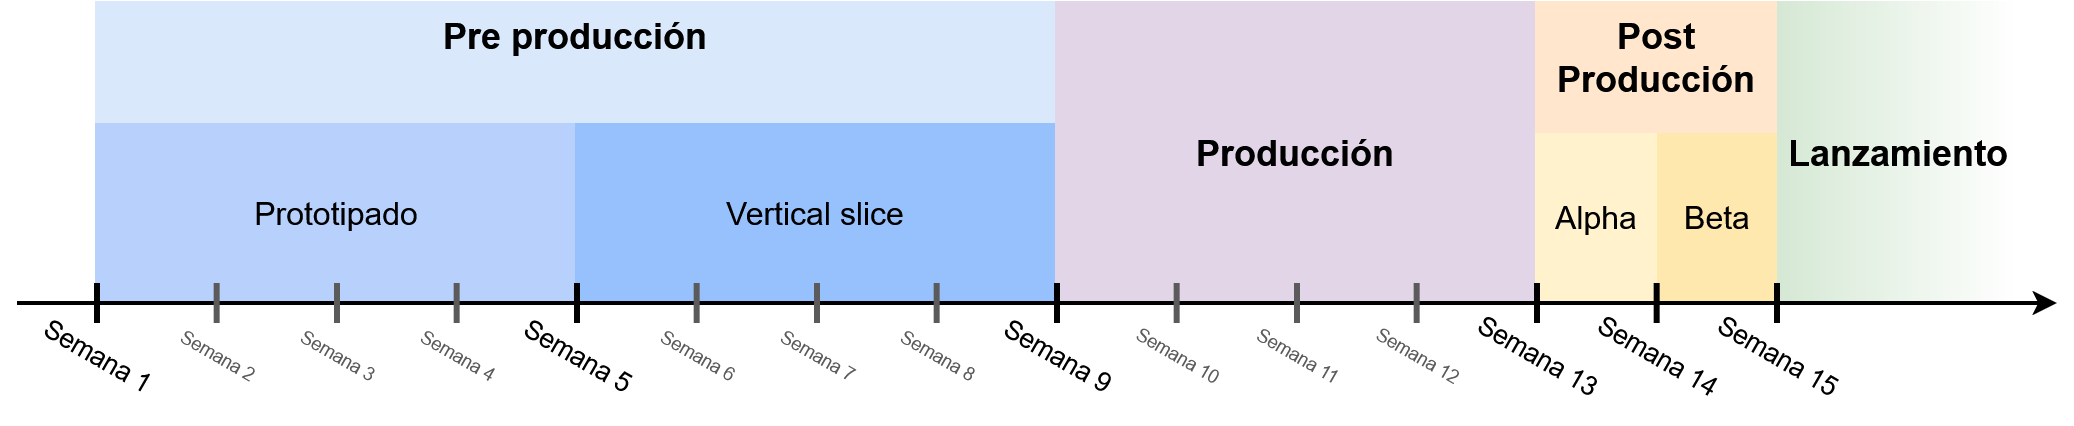
\includegraphics[width=\textwidth]{work_plan.png}
  \caption{Etapas del plan de trabajo. Creada por autor.}
  \label{fig:x plan de trabajo} 
\end{figure}
%